%Este trabalho está licenciado sob a Licença Atribuição-CompartilhaIgual 4.0 Internacional Creative Commons. Para visualizar uma cópia desta licença, visite http://creativecommons.org/licenses/by-sa/4.0/deed.pt_BR ou mande uma carta para Creative Commons, PO Box 1866, Mountain View, CA 94042, USA.

\documentclass[12pt]{article}

\input ../preambulo.tex

\lstset { %
  language=Python,
}

\newtheorem{exr}{Exercício}[section]

\usepackage{url}

\makeindex

\begin{document}

\title{Minicurso de Python para Matemática}
\author{Pedro H A Konzen}
\date{\today}
% \ifishtml
% \else
% \addcontentsline{toc}{chapter}{Capa}
% \fi

\maketitle

\tableofcontents

\section*{Licença}\label{sec_licenca}

Este trabalho é uma adaptação livre a partir está licenciado sob a Licença Atribuição-CompartilhaIgual 4.0 Internacional Creative Commons. Para visualizar uma cópia desta licença, visite http://creativecommons.org/licenses/by-sa/4.0/deed.pt\_BR ou mande uma carta para Creative Commons, PO Box 1866, Mountain View, CA 94042, USA.


\section{Sobre a linguagem}\label{sec_sobrepy}

{\python} é uma linguagem de programação de alto nível e multi-paradigma. Ou seja, é relativamente próxima das linguagens humanas naturais, é desenvolvida para aplicações diversas e permite a utilização de diferentes paradigmas de programação (programação estruturada, orientada a objetos, orientada a eventos, paralelização, etc.).

\begin{itemize}
\item Site oficial: \href{https://www.python.org/}{https://www.python.org/}
\end{itemize}

\subsection{Instalação e execução}

Para executar um código {\python} é necessário instalar um interpretador. No \href{https://www.python.org/}{site oficial do \python} estão disponíveis para {\it download} interpretadores gratuitos e com licença livre para uso. Neste minicurso, vamos utilizar {\python} 3 instalado em um sistema \verb+Linux+. Para outros sistemas, pode ser necessário fazer algumas pequenas adequações.

\subsubsection{Console online}

Alternativamente, há consoles online {\python} disponíveis na web. Para quem tem conta \href{https://www.google.com}{Google}, o \href{https://colab.research.google.com}{Google Colab} disponibiliza um \emph{notebook} {\python} gratuito. 

\subsection{Utilização}

A execução de códigos \python pode ser feita de três formas básicas:
\begin{itemize}
\item em modo iterativa em um console \python;
\item por execução de um código \verb+.py+ em um console \python;
\item por execução de um cógido \verb+.py+ em um terminal;
\end{itemize}

\begin{ex}
  Implemente o seguinte pseudocódigo.
\begin{verbatim}
s = "Ola, mundo!".
imprime(s). (imprime a string s)
\end{verbatim}
  \begin{enumerate}[a)]
  \item em modo iterativo no console;
  \item escrevendo o código \verb+.py+ e executando-o no console;
  \item escrevendo o código \verb+.py+ e executando-o no terminal.
  \end{enumerate}
  
  \noindent{\bf Resolução.} Seguem as implementações em cada caso.

  \begin{enumerate}[a)]
  \item Em modo iterativo.

    Iniciamos um console {\python} em terminal digitando
\begin{verbatim}
$ python3
\end{verbatim}
    Então, digitamos
    \begin{lstlisting}[xleftmargin=-3em]
    >>> s = "Ola, Mundo!"
    >>> print(s) #imprime a string s
    Ola, Mundo!
    \end{lstlisting}
    Para encerrar o console, digitamos
    \begin{lstlisting}[xleftmargin=-3em]
    >>> quit()
    \end{lstlisting}
    
  \item Executando {\it script} \verb+.py+ no console.

    Primeiramente, escrevemos o código
    \begin{lstlisting}
    s = "Ola, Mundo!"
    print(s) # imprime a string s
    \end{lstlisting}
    em um editor de texto (ou no seu IDE de preferência) e salvamo-lo em \verb+/pasta/codigo.py+. Então, executamo-lo no console {\python} com
    \begin{lstlisting}[xleftmargin=-3em]
    >>> exec(open('/pasta/codigo.py').read())
    Ola, mundo!
    \end{lstlisting}

  \item Executando o código em terminal.

    Considerando que já temos o código salvo em \verb+/pasta/codigo.py+, executamo-lo com
\begin{verbatim}
$ python3 /pasta/codigo.py
Olá, mundo!
\end{verbatim}
  \end{enumerate}
\end{ex}

\section{Elementos da linguagem}\label{sec_elem}

{\python} é uma linguagem de programação dinâmica em que as variáveis são declaradas automaticamente ao receberem um valor. Por exemplo, consideremos as seguintes instruções
\begin{lstlisting}
>>> x = 1
>>> y = x * 2.0
\end{lstlisting}
Na primeira instrução, a variável \lstinline+x+ é recebe o valor inteiro $1$ e, então, é armazenado na memória do computador como um objeto da classe \lstinline+int+. Na segunda instrução, \lstinline+y+ recebe o valor decimal $2.0$ (resultado de $1\times 2.0$) e é armazenado como um objeto da classe \lstinline+float+ (ponto flutuante de 64-{\it bits}). Podemos verificar isso, com as seguintes instruções
\begin{lstlisting}
>>> print(x, y)
1 2.0
>>> print(type(x), type(y))
<class 'int'> <class 'float'>
\end{lstlisting}

Códigos {\python} admitem comentários e continuação de linha como no seguinte exemplo
\begin{lstlisting}
>>> # isso eh um comentario
>>> s = "isso eh uma \
... string"
>>> print(s)
isso eh uma string
>>> type(s)
<class 'str'>
\end{lstlisting}

\begin{obs}(Notação científica)
  O {\python} aceita notação científca, por exemplo $5.2\times 10^{-2}$ é digitado como
  \begin{lstlisting}
  >>> 5.2e-2
  0.052
  \end{lstlisting}
\end{obs}

\begin{obs}
  Além dos tipos numéricos e {\it string}, {\python} também conta com os tipos de dados \lstinline+list+ (lista), \lstinline+tuple+ ($n$-upla) e \lstinline+dict+ (dicionário). Estudaremos estes tipos mais adiante neste minicurso.
\end{obs}

\begin{exr}
  Antes de implementar, diga qual o valor \lstinline+x+ após as seguintes instruções.
  \begin{lstlisting}
  >>> x = 1
  >>> y = x
  >>> y = 0
  \end{lstlisting}
  Justifique seu resposta e verifique-a.
\end{exr}

\begin{exr}
  Implemente um código em que o usuário entre com valores para as variáveis \lstinline+x+ e \lstinline+y+\footnote{A entrada de valores via console pode ser feita com a função {\python} \lstinline+input+. Consule \href{https://docs.python.org/3/library/functions.html\#input}{Python Docs}.}. Então, os valores das variáveis são permutados entre si.
\end{exr}


\subsection{Operações aritméticas elementares}

Os operadores aritméticos elementares são:
\begin{itemize}
\item[]\lstinline-+-: adição
\item[]\lstinline+-+: subtração
\item[]\lstinline+*+: multiplicação
\item[]\lstinline+/+: divisão
\item[]\lstinline+**+: potenciação
\item[]\lstinline+%+: módulo
\item[]\lstinline+//+: módulo
\end{itemize}

Consideremos o seguinte exemplo
\begin{lstlisting}
>>> 2+8*3/2**2-1
7.0
\end{lstlisting}
Observamos que as operações \lstinline+**+ tem precedência sobre as operações \lstinline+*, /+, as quais têm precedência sobre as operações \lstinline!+, -!. Operações de mesma precedência seguem a ordem da esquerda para direita, conforme escritas na linha de comando. Usa-se parênteses para alterar a precedência entre as operações, por exemplo
\begin{lstlisting}
>>> (2+8*3)/2**2-1
5.5
\end{lstlisting}
Consulte mais informações sobre a precedência de operadores em \href{https://docs.python.org/3/reference/expressions.html#operator-precedence}{Python Docs}.

\begin{exr}
  Compute as raízes do seguinte polinômio quadrático
  \begin{equation}
    x^2 - x - 2
  \end{equation}
  usando a fórmula de Bhaskara\footnote{Bhaskara Akaria, 1114 - 1185, matemático e astrônomo indiano. Fonte: \href{https://pt.wikipedia.org/wiki/Bhaskara\_II}{Wikipédia}.}
\end{exr}

O operador \lstinline+%+ módulo computa o resto da divisão e o operador \lstinline+//+ a divisão inteira, por exemplo
\begin{lstlisting}
>>> 5 % 2
1
>>> 5 // 2
2
\end{lstlisting}

\begin{exr}
  Use o {\python} para verificar se $14/21$ é menor que $15/23$. Então, compute o resto da divisão do maior quociente.
\end{exr}

\subsection{Funções e constantes elementares}

O módulo Python \href{https://docs.python.org/3/library/math.html}{math} disponibiliza várias funções e constantes elementares. Para usá-las, precisamos importar o módulo para nossa seção. Fazemos isso com a instrução
\begin{lstlisting}
>>> import math
\end{lstlisting}
Com isso, temos acesso a todas as definições e declarações contidas neste módulo. Por exemplo
\begin{lstlisting}
>>> math.pi
3.141592653589793
>>> math.cos(math.pi)
-1.0
>>> math.sqrt(2)
1.4142135623730951
>>> math.log(math.e)
1.0
\end{lstlisting}

\begin{obs}
  Notemos que \lstinline+math.log+ é a função logaritmo natural, i.e. $\ln(x) = \log_e(x)$. A implementação {\python} para o logaritmo de base 10 é \lstinline+math.log(x,10)+ ou, mais acurado, \lstinline+math.log10+.
\end{obs}

\begin{exr}
  Compute $e^{\log_3(\pi)}$.
\end{exr}

\subsection{Operadores de comparação elementares}

Os operadores de comparação elementares são
\begin{itemize}
\item[]\lstinline+==+: igual a
\item[]\lstinline+!=+: diferente de
\item[]\lstinline+>+: maior que
\item[]\lstinline+<+: menor que
\item[]\lstinline+>=+: maior ou igual que
\item[]\lstinline+<=+: menor ou igual que
\end{itemize}
Estes operadores retornam os valores lógicos \lstinline+True+ (verdadeiro) ou \lstinline+False+ (falso).

Por exemplo, temos
\begin{lstlisting}
>>> x = 2
>>> x + x == 4
True
\end{lstlisting}

\begin{exr}
  Atribua a variável \lstinline+x+ o valor $\sqrt{3}$. Então, verifique se o valor computado de $x^2$ é maior que $3$. Em caso negativo, verifique se $x^2$ é menor que 3. Comente o resultado obtido.
\end{exr}

\subsection{Operadores lógicos elementares}

Os operadores lógicos elementares são:
\begin{itemize}
\item[]\lstinline+and+: e lógico
\item[]\lstinline+or+: ou lógico
\item[]\lstinline+not+: não lógico
\end{itemize}

A tabela booleana\footnote{George Boole, 1815 - 1864, matemático e filósofo britânico. Fonte: \href{https://pt.wikipedia.org/wiki/George\_Boole}{Wikipédia}.} do ``e'' lógico é
\begin{center}
  \begin{tabular}[H]{ll|l}
    Valor & Valor & Resultado \\\hline
    True & True & True \\
    True & False & False \\
    False & True & False \\
    False & False & False \\\hline
  \end{tabular}
\end{center}
Podemos verificar isso no {\python} como segue
\begin{lstlisting}
>>> True and True
True
>>> True and False
False
>>> False and True
False
>>> False and False
False
\end{lstlisting}

\begin{exr}
  Construa as tabelas booleanas do operador \lstinline+or+ e do \lstinline+not+.
\end{exr}

\begin{exr}
  Use {\python} para verificar se $1.4 <= \sqrt{2} < 1.5$. E, também, verifique se $\sqrt{3} > 1.7$ ou $\sqrt{3} >= 1.7321$.
\end{exr}

\begin{exr}
  Implemente uma instrução para computar o operador \lstinline+xor+ (ou exclusivo). Dadas duas afirmações \lstinline+A+ e \lstinline+B+, \lstinline+A xor B+ é \lstinline+True+ no caso de uma, e somente uma, das afirmações ser \lstinline+True+, caso contrário é \lstinline+False+.
\end{exr}


\subsection{Conjuntos}

{\python} tem conjuntos finitos como um tipo básico de variável. Um conjunto é uma coleção de itens \emph{não ordenada} e \emph{imutável} e \emph{não admite itens duplicados}. Por exemplo,
\begin{lstlisting}
>>> a = {1, 2, 3}
>>> type(a)
<class 'set'>
>>> b = set((2, 1, 3, 3))
>>> b
{1, 2, 3}
>>> a == b
True
>>> # conjunto vazio
>>> e = set()
\end{lstlisting}
aloca o conjunto $a = {1,2 3}$. Note que o conjunto $b$ é igual a $a$. Observamos que o conjunto vazio deve ser construído com a instrução \lstinline+set()+ e não com \lstinline+{}+\footnote{Isso constrói um dicionário vazio, como introduziremos logo mais.}.

\begin{obs}
  A função {\python} \lstinline+len+ retorna o número de elementos de um conjunto. Por exemplo,
  \begin{lstlisting}
  >>> len(a)
  3
  \end{lstlisting}
\end{obs}

\begin{itemize}
\item Operadores envolvendo conjuntos:
  \begin{itemize}
  \item[] \lstinline+-+: diferença entre conjuntos;
  \item[] \lstinline+|+: união de conjuntos;
  \item[] \lstinline+&+: interseção de conjuntos;
  \item[] \lstinline+^+: diferença simétrica;
  \end{itemize}
\end{itemize}

\begin{ex}
  Sejam os conjuntos
  \begin{gather}
    A = \{2, \pi, -0.25, 3, \text{'banana'}\},\\
    B = \{\text{'laranja'}, 3, \operatorname{arc cos}(-1), -1\}
  \end{gather}
  Compute
  \begin{enumerate}[a)]
  \item $A\setminus B$
  \item $A\cup B$
  \item $A\cap B$
  \item $A\Delta B = (A\setminus B) \cup (B\setminus A)$
  \end{enumerate}

  \noindent{\bf Resolução.} Começamos alocando os conjuntos como segue
  \begin{lstlisting}
  >>> import math
  >>> A = {2, math.pi, -0.25, 3, 'banana'}
  >>> B = {'laranja', 3, math.acos(-1), -1}
  \end{lstlisting}
  
  \begin{enumerate}[a)]
  \item $A\setminus B$
    \begin{lstlisting}
    >>> A - B
    {-0.25, 2, 'banana'}
    \end{lstlisting}
  \item $A\cup B$
    \begin{lstlisting}
    >>> A | B
    {-0.25, 2, 3, 3.141592653589793, \
    'laranja', 'banana', -1}
    \end{lstlisting}
  \item $A\cap B$
    \begin{lstlisting}
    >>> A & B
    {3, 3.141592653589793}
    \end{lstlisting}
  \item $A\Delta B$
    \begin{lstlisting}
    >>> A ^ B
    {-0.25, 2, 'laranja', 'banana', -1}
    \end{lstlisting}
  \end{enumerate}
\end{ex}

\begin{obs}\label{obs:compreensão_de_conjuntos}
  {\python} disponibiliza a sintaxe de compreensão de conjuntos. Por exemplo,
  \begin{lstlisting}
  >>> {x for x in A if type(x) == type('')}
  {'banana'}
  \end{lstlisting}
\end{obs}

\begin{exr}
  Considere o conjunto
  \begin{equation}
    Z = {-3, -2, -1, 0, 1, 2, 3}.
  \end{equation}
  Faça um código {\python} para extrair o subconjunto dos números pares do conjunto $Z$.
\end{exr}

\subsection{$n$-uplas}

Em {\python} $n$-uplas ({\it tuples}) é uma sequência de objetos, i.e. uma coleção ordenada, indexada e imutável. Por exemplo, na sequência temos um par, uma tripla e uma quadrupla
\begin{lstlisting}
>>> a = (1, 2)
>>> a
(1, 2)
>>> b = -1, 1, 0
(-1, 1, 0)
>>> c = (0.5, 'laranja', {2, -1}, ['t', 0])
>>> c
(0.5, 'laranja', {2, -1}, ['t', 0])
>>> len(c)
4
\end{lstlisting}
A função \lstinline+len+ retorna o número de objetos da $n$-upla. Pode acessar um elemento, usando sua indexação. Por exemplo,
\begin{lstlisting}
>>> c[2]
{2, -1}
\end{lstlisting}
Pode-se também extrair uma fatia (um subconjunto) usando-se a notação \lstinline+:+. Por exemplo,
\begin{lstlisting}
>>> c[1:3]
('laranja', {2, -1})
\end{lstlisting}

\begin{itemize}
\item Operadores básicos:
  \begin{itemize}
  \item[] \lstinline-+-: concatenação
    \begin{lstlisting}
    >>> (1, 2) + (3, 4, 5)
    (1, 2, 3, 4, 5)
    \end{lstlisting}
  \item[] \lstinline+*+: repetição
    \begin{lstlisting}
    >>> (1, 2) * 2
    (1, 2, 1, 2)
    \end{lstlisting}
  \item[] \lstinline+in+: pertencimento
    \begin{lstlisting}
    >>> 1 in (-1, 0, 1, 2)
    True
    \end{lstlisting}
  \end{itemize}
\end{itemize}

\begin{exr}
  Aloque os conjuntos
  \begin{gather}
    A = \{-1, 0, 2\},\\
    B = \{2, 3, 5\}.
  \end{gather}
  Então, compute o produto cartesiano $A\times B=\{(a,b):~a\in A, b\in B\}$. Qual o número de elementos da $A\times B$? Dica: use a sintaxe de compreensão de conjuntos (consulte a Observação \ref{obs:compreensão_de_conjuntos}).
\end{exr}

\begin{exr}
  Aloque o gráfico discreto da função\footnote{O gráfico de uma função restrito a um conjunto $A$ é o conjunto $\operatorname{G}(f)|_{A} = \{(x,y):~x\in A, y=f(x)\}$.} $f(x) = x^2$ para $x=0, \frac{1}{2}, 1, 2$. Dica: use a sintaxe de compreensão de conjuntos (consulte a Observação \ref{obs:compreensão_de_conjuntos}).
\end{exr}

\subsection{Listas}

O tipo {\python} \lstinline+list+ permite alocar em uma única variável uma lista de itens ordenada. Por exemplo, observemos as seguintes listas
\begin{lstlisting}
>>> x = [-1, 2, -3, -5]
>>> type(x)
<class 'list'>
>>> y = ['a', 'b', 'a']
>>> y
['a', 'b', 'a']
>>> vazia = []
>>> len(x)
4
\end{lstlisting}

Os elementos de uma lista são indexados, o índice $0$ corresponde ao primeiro elemento, o índice $1$ ao segundo elemento e assim por diante. Desta forma é possível o acesso direto a um elemento de uma lista usando-se sua posição. Por exemplo,
\begin{lstlisting}
>>> x[0]
-1
>>> y[2] = 'c'
>>> y
['a', 'b', 'c']
\end{lstlisting}
Pode-se fazer um corte de elementos de uma lista usando o operador \lstinline+:+. Por exemplo,
\begin{lstlisting}
>>> x = [1,2,-1,3,-2]
>>> x[1:3]
[2,-1]
\end{lstlisting}

\begin{itemize}
\item Operadores básicos:
  \begin{itemize}
  \item[] \lstinline-+-: concatenação
    \begin{lstlisting}
    >>> [1, 2] + [3, 4, 5]
    [1, 2, 3, 4, 5]
    \end{lstlisting}
  \item[] \lstinline+*+: repetição
    \begin{lstlisting}
    >>> [1, 2] * 2
    [1, 2, 1, 2]
    \end{lstlisting}
  \item[] \lstinline+in+: pertencimento
    \begin{lstlisting}
    >>> 1 in [-1, 0, 1, 2]
    True
    \end{lstlisting}
  \end{itemize}
\end{itemize}

\begin{obs}
  Listas contam com várias funções prontas para a execução de diversas tarefas práticas como, por exemplo, inserir/deletar itens, contar ocorrências, ordenar itens, etc. Consulte \href{https://docs.python.org/3/tutorial/datastructures.html#more-on-lists}{Python Docs}.
\end{obs}

\begin{obs}(Alocação {\it versus} cópia)
  Estude o seguinte exemplo
  \begin{lstlisting}
  >>> x = [2, 3, 1]
  >>> y = x
  >>> y[1] = 0
  >>> x
  [2, 0, 1]
  \end{lstlisting}
  Notamos que \lstinline+y+ aponta para o mesmo endereço de memória de \lstinline+x+. Para copiar uma lista e alocá-la em um novo endereço de memória, deve-se usar a função \lstinline+list.copy()+, como segue
  \begin{lstlisting}
  >>> x = [2, 3, 1]
  >>> y = x.copy()
  >>> y[1] = 0
  >>> x
  [2, 3, 1]
  >>> y
  [2, 0, 1]
  \end{lstlisting}
\end{obs}

\begin{exr}
  Implemente uma lista para alocar os primeiros 5 elementos da sequência de Fibonacci\footnote{Leonardo Fibonacci, 1170 - 1250, matemático italiano. Fonte: \href{https://pt.wikipedia.org/wiki/Leonardo\_Fibonacci}{Wikipédia}.}.
\end{exr}

\begin{exr}
  Uma aplicação do Método Babilônico\footnote{Matemática Babilônica, matemática desenvolvida na Mesopotâmia, desde os Sumérios até a queda da Babilônia em 539 a.C.. Fonte: \href{https://pt.wikipedia.org/wiki/Matem\%C3\%A1tica\_babil\%C3\%B4nica}{Wikipédia}.} para a aproximação da solução da equação $x^2-2 = 0$, consiste na iteração
  \begin{gather}
    x_0 = 1,\\
    x_{i+1} = \frac{x_i}{2} + \frac{1}{x_i},\quad i=0,1,2,\ldots
  \end{gather}
  Implemente uma lista para alocar as quatro primeiras aproximações da solução, i.e. $x_0$, $x_1$, $x_2$, $x_3$.
\end{exr}

\begin{exr}
  Aloque os seguintes vetores como listas no {\python}
  \begin{gather}
    x = (-1, 3, -2),\\
    y = (4, -2, 0).
  \end{gather}
  Então, compute
  \begin{enumerate}[a)]
  \item $x+y$
  \item $x\cdot y$
  \end{enumerate}
\end{exr}

\begin{exr}
  Uma matriz pode ser alocada como uma lista de listas {\python}, alocando cada linha como uma lista e a matriz como a lista destas listas. Por exemplo, a matriz
  \begin{equation}
    M =
    \begin{bmatrix}
      1 & -2 \\
      2 & 3
    \end{bmatrix}
  \end{equation}
  pode ser alocada como a seguinte lista de listas
  \begin{lstlisting}
  >>> M = [[1,-2],[2,3]]
  >>> M
  [[1, -2], [2, 3]]
  \end{lstlisting}
  Use listas para alocar a matriz
  \begin{equation}
    A =
    \begin{bmatrix}
      1 & -2 & 1\\
      8 & 0 & -7\\
      3 & -1 & -2
    \end{bmatrix}
  \end{equation}
  e o vetor coluna
  \begin{equation}
    x = (2, -3, 1),
  \end{equation}
  então compute $Ax$ e $x^TA$.
\end{exr}

\subsection{Dicionários}

Em {\python} um dicionário é um mapeamento objeto a objeto, cada par (chave:valor) é separado por uma vírgula. Por exemplo,
\begin{lstlisting}
>>> a = {'nome': 'triangulo', 'perimetro': 3.2}
>>> a
{'nome': 'triangulo', 'perimetro': 3.2}
>>> b = {1: 2.71, (1,2): 2, 'a': {1,0,-1}}
>>> b
{1: 2.71, (1, 2): 2, 'a': {0, 1, -1}}
>>> d = {1: 'a', 'b': 2, 1.4: -1, 2: 'b'}
>>> d
{1: 'a', 'b': 2, 1.4: -1, 2: 'b'}
\end{lstlisting}

O acesso a um item do dicionário é feito usando-se sua \emph{chave}. Por exemplo,
\begin{lstlisting}
>>> d['b']
2
>>> d[1.4] = 1
>>> d
{1: 'a', 'b': 2, 1.4: 1, 2: 'b'}
\end{lstlisting}
Pode-se adicionar um novo par, simplesmente, atribuindo valor a uma nova chave. Por exemplo,
\begin{lstlisting}
>>> d[1.5] = 0
>>> d
{1: 'a', 'b': 2, 1.4: 1, 2: 'b', 1.5: 0}
\end{lstlisting}

\begin{obs}
  Consulte sobre mais sobre dicionários em \href{https://docs.python.org/3/tutorial/datastructures.html#dictionaries}{Python Docs}.
\end{obs}

\begin{exr}
  Considere a função afim
  \begin{equation}
    f(x) = 3 - x.
  \end{equation}
  Implemente um dicionário para alocar a raiz da função, a interseção com o eixo $y$ e seu coeficiente angular.
\end{exr}

\begin{exr}
  Considere a função quadrática
  \begin{equation}
    g(x) = x^2 - x - 2
  \end{equation}
  Implemente um dicionário para alocar suas raízes, vértice e interseção com o eixo $y$.
\end{exr}

\section{Função, ramificação e repetição}\label{sec_fun}

Nesta seção, vamos introduzir funções e estruturas de ramificação e de repetição. Estes são procedimentos fundamentais na programação estruturada.

\subsection{Definindo funções}

Em {\python}, uma função é definida com a palavra-chave \lstinline+def+ seguida de seu nome e seus parâmetros encapsulados entre parênteses e por dois-pontos \lstinline+:+. Suas instruções formam o corpo da função, iniciam-se na linha abaixo e devem estar indentadas. A indentação define o escopo da função. Por exemplo, a seguinte função imprime o valor da função
\begin{equation}
  f(x) = 2x - 3
\end{equation}
\begin{lstlisting}
>>> def f(x):
...     y = 2*x - 3
...     print(y)
... 
>>> f(2)
1
\end{lstlisting}
Você pode protestar que \lstinline+f+ não é uma função e, sim, um procedimento, pois não retorna valor. Para uma função retornar um objeto, usamos a instrução \lstinline+return+. Por exemplo,
\begin{lstlisting}
>>> def f(x):
...     y = 2*x - 3
...     return y
... 
>>> z = f(2)
>>> z
1
\end{lstlisting}

\begin{obs}
  Para funções pequenas, pode-se utilizar a instrução \lstinline+lambda+ de funções anônimas. Por exemplo,
  \begin{lstlisting}
  >>> f = lambda x: 2*x - 3
  >>> f(3)
  3
  \end{lstlisting}
\end{obs}

\begin{obs}
  Consulte mais informações sobre a definição de funções em \href{https://docs.python.org/3/tutorial/controlflow.html#defining-functions}{Python Docs}.
\end{obs}

\begin{exr}
  Implemente uma função para computar as raízes de uma polinômio de grau 1 $p(x) = ax + b$.
\end{exr}

\begin{exr}
  Implemente uma função para computar as raízes de uma polinômio de grau 2 $p(x) = ax^2 + bx + c$.
\end{exr}

\begin{exr}
  Implemente uma função que computa o produto escalar de dois vetores
  \begin{gather}
    x = (x_0, x_1, x_2),\\
    y = (y_0, y_1, y_2).
  \end{gather}
  Use listas para representar os vetores no {\python}.
\end{exr}

\begin{exr}
  Implemente uma função que computa o determinante de matrizes $2\times 2$. Use lista de listas para representar as matrizes.
\end{exr}

\begin{exr}
  Implemente uma função que computa a multiplicação matrix-vetor $Ax$, com $A$ $2\times 2$ e $x$ um vetor coluna de dois elementos.
\end{exr}

\begin{exr}(Recursividade) Implemente uma função recursiva para computar o fatorial de um número natural $n$, i.e. $n!$.  
\end{exr}

\subsection{Ramificação}

Uma estrutura de ramificação é uma instrução para a tomada de decisões durante a execução de um programa. No {\python}, está disponível a instrução \lstinline+if+. Consultemos o seguinte exemplo.
\begin{lstlisting}
def paridade(n):
    if (n%2 == 0):
        print('par')
\end{lstlisting}
Aqui, a função \lstinline+paridade+ recebe o valor \lstinline+n+. Se (\lstinline+if+) o resto da divisão de \lstinline+n+ por 2 é igual a zero (condição), então (\lstinline+:+) imprime a {\it string} \lstinline+par+.

\begin{obs}
  A indentação determina o escopo de cada instrução \lstinline+if+.
\end{obs}

Também está disponível a instrução \lstinline+if-else+. Por exemplo,
\begin{lstlisting}
def paridade(n):
    if (n%2 == 0):
        print('par')
    else:
        print('impar')    
\end{lstlisting}
Agora, se (\lstinline+if+) a condição \lstinline!(n%2 == 0)! for verdadeira (\lstinline+True+), então imprime \lstinline+par+, senão (\lstinline+else+) imprime \lstinline+impar+.

Ainda, é possível ter instruções \lstinline+if-else+ encadeadas. Por exemplo,
\begin{lstlisting}
def paridade(n):
     if (n%2 == 0):
          print('eh divisivel por 2')
     elif (n%3 == 0):
          print('eh divisivel por 3')
     else:
          print('nao eh divisivel por 2 e 3')    
\end{lstlisting}
Observe que \lstinline+elif+ deve ser utilizado no lugar de \lstinline+else if+.

\begin{exr}
  Implemente uma função que recebe dois números $n$ e $m$ e imprime o maior deles.
\end{exr}

\begin{exr}
  Implemente uma função que recebe os coeficientes de um polinômio
  \begin{equation}
    p(x) = ax^2 + bx + c
  \end{equation}
  e classifique-o como um polinômio de grau 0, 1 ou 2.
\end{exr}

\subsection{Repetição}

Estruturas de repetição são instruções que permitem que a execução repetida de uma região do código. São duas instruções disponível \lstinline+while+ e \lstinline+for+.

\subsubsection{while}

A sintaxe da instrução \lstinline+while+ é
\begin{lstlisting}
while expressao:
     comando 0
     .
     .
     .
     comando n
\end{lstlisting}
Isto é, enquanto (\lstinline+while+) a expressão (\lstinline+expressao+) for verdadeira, os comandos \lstinline+comando 0+ a \lstinline+comando n+ serão repetidamente executados em ordem. Por exemplo, o seguinte código computa a soma dos $10$ primeiros números naturais e, então imprime-a.
\begin{lstlisting}
n = 0
s = 0
while (n < 10):
    s += n
    n += 1
print(s)
\end{lstlisting}

\begin{obs}
  As instruções de controle \lstinline+break+, \lstinline+continue+ são bastante úteis em várias situações. A primeira, encerra as repetições e, a segunda, pula para uma nova repetição. Consulte mais em \href{https://docs.python.org/3/tutorial/controlflow.html\#break-and-continue-statements-and-else-clauses-on-loops}{Python Docs}.
\end{obs}

\begin{exr}
  Use \lstinline+while+ para imprimir os dez primeiros números ímpares.
\end{exr}

\begin{exr}
  Uma aplicação do Método Babilônico\footnote{Matemática Babilônica, matemática desenvolvida na Mesopotâmia, desde os Sumérios até a queda da Babilônia em 539 a.C.. Fonte: \href{https://pt.wikipedia.org/wiki/Matem\%C3\%A1tica\_babil\%C3\%B4nica}{Wikipédia}.} para a aproximação da solução da equação $x^2-2 = 0$, consiste na iteração
  \begin{gather}
    x_0 = 1,\\
    x_{i+1} = \frac{x_i}{2} + \frac{1}{x_i},\quad i=0,1,2,\ldots
  \end{gather}
  Faça um código com \lstinline+while+ para computar aproximação $x_{i}$, tal que $|x_{i}-x_{i-1}|<10^{-5}$.
\end{exr}

\subsubsection{for}

A estrutura \lstinline+for+ tem a sintaxe
\begin{lstlisting}
  for i in iteravel:
      escopo
\end{lstlisting}
onde, \lstinline+iteravel+ pode ser qualquer objeto de uma classe iterável (conjunto, $n$-upla, lista, dicionário, {\it string}). Os comandos dentro do escopo (determinado pela indentação) são repetidos para cada iterada \lstinline+i+. Por exemplo,
\begin{lstlisting}
>>> for i in [0,1,2]:
...     print(i)
... 
0
1
2
\end{lstlisting}

\subsubsection{range}

A função {\python} \lstinline+range([start,]stop[,sep])+ é particularmente útil na construção de instruções \lstinline+for+. Ela cria um objeto de classe iterável de \lstinline+start+ (incluído) a \lstinline+stop+ (excluído), de elementos igualmente separados por \lstinline+sep+. Por padrão, \lstinline+start=0+, \lstinline+sep=1+ caso omitidos. Por exemplo,
\begin{lstlisting}
>>> for i in range(1,6,2):
...     print(i)
... 
1
3
5
\end{lstlisting}
ou
\begin{lstlisting}
>>> for i in range(3):
...     print(i)
... 
0
1
2
\end{lstlisting}

\begin{exr}
  Escreva uma função que retorne o $n$-ésimo termo da função de Fibonacci\footnote{Leonardo Fibonacci, 1170 - 1250, matemático italiano. Fonte: \href{https://pt.wikipedia.org/wiki/Leonardo\_Fibonacci}{Wikipédia}.}, $n\geq 1$. 
\end{exr}

\begin{exr}
  Implemente uma função para computar o produto escalar de dois vetores de $n$ elementos. Assuma que os vetores estão alocados em listas.
\end{exr}

\begin{exer}
  Implemente uma função para computar a multiplicação de uma matriz $A$ $n\times n$ por um vetor coluna $x$ de $n$ elementos. Assuma que o vetor está alocada como uma lista e a matriz como uma lista de listas por linhas.
\end{exer}

\begin{exer}
  Implemente uma função para computar a multiplicação de uma matriz $A$ $n\times m$ por uma matriz $B$ de $m\times n$. Assuma que as matrizes estão alocadas como listas de listas por linhas de cada matriz.
\end{exer}

\section{Elementos da computação matricial}\label{sec_mat}

Nesta seção, vamos explorar a \href{https://numpy.org/}{NumPy} (Numerical Python), biblioteca para tratamento numérico de dados. Ela é extensivamente utilizada nos mais diversos campos da ciência e da engenharia. Aqui, vamos nos restringir a introduzir algumas de suas ferramentas para a computação matricial.

Usualmente, a biblioteca é importada como segue
\begin{lstlisting}
>>> import numpy as np
\end{lstlisting}

\subsection{NumPy array}

Um \lstinline+array+ é uma tabela de valores (vetor, matriz ou multidimensional) e contém informação sobre os dados brutos, indexação e como interpretá-los. {\bf Os elementos são todos do mesmo tipo} (diferente de uma lista Python), referenciados pela propriedade \lstinline+dtype+. A indexação dos elementos pode ser feita por um \lstinline+tuple+ de inteiros não negativos, por booleanos, por outro \lstinline+array+ ou por números inteiros. O \lstinline+rank+ de um \lstinline+array+ é seu número de dimensões (chamadas de \lstinline+axes+\footnote{Do inglês, plural de {\it axis}, eixo.}). O \lstinline+shape+ é um \lstinline+tuple+ de inteiros que fornece seu tamanho (número de elementos) em cada dimensão. Sua inicialização pode ser feita usando-se listas simples ou encadeadas. Por exemplo,
\begin{lstlisting}
>>> a = np.array([1,3,-1,2])
>>> print(a)
[ 1  3 -1  2]
>>> a.dtype
dtype('int64')
>>> a.shape
(4,)
>>> a[2]
-1
>>> a[1:3]
array([ 3, -1])
\end{lstlisting}
temos um \lstinline+array+ de números inteiros com quatro elementos dispostos em um único \lstinline+axis+ (eixo). Podemos interpretá-lo como uma representação de um vetor linha ou coluna, i.e.
\begin{equation}
  a = (1, 3, -1, 2)
\end{equation}
vetor coluna ou $a^T$ vetor linha.

Outro exemplo,
\begin{lstlisting}
>>> a = np.array([[1.0,2,3],[-3,-2,-1]])
>>> a.dtype
dtype('float64')
>>> a.shape
(2, 3)
>>> a[1,1]
-2.0
\end{lstlisting}
temos um \lstinline+array+ de números decimais (\lstinline+float+) dispostos em um arranjo com dois \lstinline+axes+ (eixos). O primeiro \lstinline+axis+ tem tamanho $2$ e o segundo tem tamanho $3$. Ou seja, podemos interpretá-lo como uma matriz de duas linhas e três colunas. Podemos fazer sua representação algébrica como
\begin{equation}
  a =
  \begin{bmatrix}
    1 & 2 & 3\\
    -3 & -2 & -1 
  \end{bmatrix}
\end{equation}

\subsubsection{Inicialização de um array}\label{subsubsection:iniarray}

O \href{https://numpy.org/}{NumPy} conta com úteis funções de inicialização de \lstinline+array+. Vejam algumas das mais frequentes:
\begin{itemize}
\item \lstinline+np.zeros()+: inicializa um \lstinline+array+ com todos seus elementos iguais a zero.
  \begin{lstlisting}
  >>> np.zeros(2)
  array([0., 0.])
  \end{lstlisting}
\item \lstinline+np.ones()+: inicializa um \lstinline+array+ com todos seus elementos iguais a $1$.
  \begin{lstlisting}
  >>> np.ones((3,2), dtype='int')
  array([[1, 1],
         [1, 1],
         [1, 1]])
  \end{lstlisting}
\item \lstinline+np.empty()+: inicializa um \lstinline+array+ sem alocar valores para seus elementos\footnote{Atenção! Os valores dos elementos serão dinâmicos conforme ``lixo'' da memória.}.
  \begin{lstlisting}
  >>> np.empty(3)
  array([4.9e-324, 1.5e-323, 2.5e-323])
  \end{lstlisting}
\item \lstinline+np.arange()+: inicializa um \lstinline+array+ com uma sequência de elementos\footnote{Similar a função Python \lstinline+range+.}.
  \begin{lstlisting}
  >>> np.arange(1,6,2)
  array([1, 3, 5])
  \end{lstlisting}
\item \lstinline+np.linspace(a, b[, num=n])+: inicializa um \lstinline+array+ como uma sequência de elementos que começa em \lstinline+a+, termina em \lstinline+b+ (incluídos) e contém \lstinline+n+ elementos igualmente espaçados.
  \begin{lstlisting}
  >>> np.linspace(0, 1, num=5)
  array([0.  , 0.25, 0.5 , 0.75, 1.  ])
  \end{lstlisting}
\end{itemize}

\subsubsection{Manipulação de arrays}

Outras duas funções importantes no tratamento de \lstinline+arrays+ são:
\begin{itemize}
\item \lstinline+arr.reshape()+: permite a alteração da forma de um \lstinline+array+.
  \begin{lstlisting}
  >>> a = np.array([-2,-1])
  >>> a
  array([-2, -1])
  >>> a.reshape(2,1)
  array([[-2],
         [-1]])
  \end{lstlisting}

   O \lstinline+arr.reshape()+ também permite a utilização de um coringa \lstinline+-1+ que será dinamicamente determinado de forma obter-se uma estrutura adequada. Por exemplo,
   \begin{lstlisting}
   >>> a = np.array([[1,2],[3,4]])
   >>> a
   array([[1, 2],
          [3, 4]])
   >>> a.reshape((-1,1))
   array([[1],
          [2],
          [3],
          [4]])
   \end{lstlisting}
\item \lstinline+arr.transpose()+: computa a transposta de uma matriz.
    \begin{lstlisting}
    >>> a = np.array([[1,2],[3,4]])
    >>> a
    array([[1, 2],
           [3, 4]])
    >>> a.transpose()
    array([[1, 3],
           [2, 4]])
    \end{lstlisting}
 \item \lstinline+np.concatenate()+: concatena \lstinline+arrays+.
   \begin{lstlisting}
   >>> a = np.array([1,2])
   >>> b = np.array([2,3])
   >>> c = np.concatenate((a,b))
   >>> c
   array([1, 2, 2, 3])
   >>> a = a.reshape((1,-1))
   >>> a.ndim
   2
   >>> b = b.reshape((1,-1))
   >>> b
   array([[2, 3]])
   >>> d = np.concatenate((a,b), axis=0)
   >>> d
   array([[1, 2],
          [2, 3]])
   \end{lstlisting}
\end{itemize}

\subsubsection{Operadores elemento-a-elemento}\label{subsubsection:ope-a-e}

Os operadores aritméticos disponível no Python atuam elemento-a-elemento nos \lstinline+arrays+. Por exemplo,
\begin{lstlisting}
>>> a = np.array([1,2])
>>> b = np.array([2,3])
>>> a+b
array([3, 5])
>>> a-b
array([-1, -1])
>>> b*a
array([2, 6])
>>> a**b
array([1, 8])
>>> 2*b
array([4, 6])
\end{lstlisting}

O \href{https://numpy.org/}{NumPy} também conta com várias funções matemáticas elementares que operam elemento-a-elemento em \lstinline+arrays+. Por exemplo,
\begin{lstlisting}
>>> a = np.array([np.pi, np.sqrt(2)])
>>> a
array([3.14159265, 1.41421356])
>>> np.sin(a)
array([1.22464680e-16, 9.87765946e-01])
>>> np.exp(a)
array([23.14069263,  4.11325038])
\end{lstlisting}
 
\begin{obs}
O \href{https://numpy.org/}{NumPy} contém um série de outras funções práticas para a manipulação de \lstinline+arrays+. Consulte \href{https://numpy.org/doc/stable/user/absolute_beginners.html\#numpy-the-absolute-basics-for-beginners}{NumPy: the absolute basics for beginners}.  
\end{obs}

\subsection{Elementos da álgebra linear}

O \href{https://numpy.org/}{NumPy} conta com um módulo de álgebra linear
\begin{lstlisting}
>>> from numpy import linalg
\end{lstlisting}

\subsection{Vetores}

Um vetor podem ser representado usando um \lstinline+array+ de um eixo (dimensão) ou um com dois eixos, caso se queira diferenciá-lo entre um vetor linha ou coluna. Por exemplo, os vetores
\begin{equation}
  a = (2, -1, 7),\\
  b = (3, 1, 0)^T
\end{equation}
podem ser alocados com
\begin{lstlisting}
>>> x = np.array([2,-1,7])
>>> y = np.array([3,1,0])
\end{lstlisting}
Caso queira-se que $x$ siga um arranjo em coluna, pode-se modificado como segue
\begin{lstlisting}
>>> a = a.reshape((-1,1))
>>> a
array([[ 2],
       [-1],
       [ 7]])
\end{lstlisting}

Como já vimos, o \href{https://numpy.org/}{NumPy} conta com operadores elemento-a-elemento que podem ser utilizados na álgebra envolvendo \lstinline+arrays+, logo também aplicáveis a vetores (consulte a Subseção \ref{subsubsection:ope-a-e}). Vamos, aqui, introduzir outras operações próprias deste tipo de objeto.

\begin{exr}
  Aloque cada um dos seguintes vetores como um \href{https://numpy.org/}{NumPy} \lstinline+array+:
  \begin{enumerate}
  \item[a)] $x = (1.2, -3.1, 4)$
  \item[b)] $y = x^T$
  \item[c)] $z = (\pi, \sqrt{2}, e^{-2})^T$
  \end{enumerate}
\end{exr}

\subsubsection{Produto escalar e norma}

Dados dois vetores,
\begin{gather}
  x = (x_0, x_1, \dotsc, x_{n-1}),\\
  y = (y_0, y_1, \dotsc, y_{n-1})
\end{gather}
define-se o \emph{produto escalar} por
\begin{equation}
  x\cdot y = x_0y_0 + x_1y_1 + \cdots + x_{n-1}y_{n-1}
\end{equation}
Com o \href{https://numpy.org/}{NumPy}, podemos computá-lo com a função \lstinline+np.dot()+. Por exemplo,
\begin{lstlisting}
>>> x = np.array([-1, 0, 2, 4])
>>> y = np.array([0, 1, 1, -1])
>>> np.dot(x,y)
-2
\end{lstlisting}

A norma (euclidiana) de um vetor é definida por
\begin{equation}
  \|x\| = \sqrt{\sum_{i=0}^{n-1} x_i^2}.
\end{equation}
O \href{https://numpy.org/}{NumPy} conta com a função \lstinline+np.linalg.norm()+ para computá-la. Por exemplo,
\begin{lstlisting}
  >>> np.linalg.norm(y)
  1.7320508075688772
\end{lstlisting}

\begin{exr}
  Faça um código para computar o produto escalar $x\cdot y$ sendo
  \begin{gather}
    x = (1.2, \ln(2), 4),\\
    y = (\pi^2, \sqrt{3}, e)
  \end{gather}
\end{exr}


\subsection{Matrizes}

Uma matriz pode ser alocada como um \href{https://numpy.org/}{NumPy} \lstinline+array+ de dois eixos (dimensões). Por exemplo, as matrizes
\begin{gather}
  A =
  \begin{bmatrix}
    2 & -1 & 7\\
    3 & 1 & 0
  \end{bmatrix},\\
  B =
  \begin{bmatrix}
    4 & 0\\
    2 & 1\\
   -8 & 6
  \end{bmatrix}
\end{gather}
podem ser alocadas como segue
\begin{lstlisting}
>>> A = np.array([[2,-1,7],[3,1,0]])
>>> A
array([[ 2, -1,  7],
       [ 3,  1,  0]])
>>> B = np.array([[4,0],[2,1],[-8,6]])
>>> B
array([[ 4,  0],
       [ 2,  1],
       [-8,  6]])
\end{lstlisting}


Como já vimos, o \href{https://numpy.org/}{NumPy} conta com operadores elemento-a-elemento que podem ser utilizados na álgebra envolvendo \lstinline+arrays+, logo também aplicáveis a matrizes (consulte a Subseção \ref{subsubsection:ope-a-e}). Vamos, aqui, introduzir outras operações próprias deste tipo de objeto.

\begin{exr}
  Aloque cada uma das seguintes matrizes como um Numpy \lstinline+array+:
  \begin{exr}
  \item[a)]
    \begin{equation}
      A =
      \begin{bmatrix}
        -1 & 2\\
        2 & -4\\
        6 & 0
      \end{bmatrix}
    \end{equation}
  \item[b)] $B = A^T$ 
  \end{exr}
\end{exr}

\begin{exr}
  Seja
  \begin{lstlisting}
  >>> A = np.array([[2,1],[1,1],[-3,-2]])
  \end{lstlisting}
  Determine o formato (\lstinline+shape+) dos seguintes \lstinline+arrays+:
  \begin{enumerate}[a)]
  \item \lstinline+A[:,0]+
  \item \lstinline+A[:,0:1]+
  \item \lstinline+A[1:3,0]+
  \item \lstinline+A[1:3,0:1]+
  \item \lstinline+A[1:3,0:2]+
  \end{enumerate}
\end{exr}

\subsubsection{Inicialização de matrizes}

Além das inicializações de \lstinline+arrays+ já estudadas na Subseção \ref{subsubsection:iniarray}, temos mais algumas que são particularmente úteis no caso de matrizes.
\begin{itemize}
\item \lstinline+np.eye(n)+: retorna a matriz identidade $n\times n$.
  \begin{lstlisting}
  >>> np.eye(3)
  array([[1., 0., 0.],
         [0., 1., 0.],
         [0., 0., 1.]])
   \end{lstlisting}
 \item \lstinline+np.diag(v)+: retorna uma matriz diagonal formada pela \lstinline+list v+.
   \begin{lstlisting}
   >>> np.diag([1,2,3])
   array([[1, 0, 0],
          [0, 2, 0],
          [0, 0, 3]])
   \end{lstlisting}
 \end{itemize}

 \begin{exr}
   Aloque a matriz escalar $C = [c_{ij}]_{i,j=0}^{99}$, sendo $c_{ii}=\pi$ e $c_{ij}=0$ para $i\neq j$.
 \end{exr}

\subsubsection{Multiplicação de matrizes}

A multiplicação da matriz $A = [a_{ij}]_{i,j=0}^{n-1,l-1}$ pela matriz $B = [b_{ij}]_{i,j=0}^{l-1,m-1}$ e a matriz $C = AB = [c_{ij}]_{i,j=0}^{n-1,m-1}$ tal que
\begin{equation}
  c_{ij} = \sum_{k=0}^{l-1} a_{ik}b_{k,j}
\end{equation}
O \href{https://numpy.org/}{NumPy} tem a função \lstinline+np.matmul()+ para computar a multiplicação de matrizes. Por exemplo,
\begin{lstlisting}
>>> C = np.matmul(A,B)
>>> C
array([[-50,  41],
       [ 14,   1]])
\end{lstlisting}

\begin{obs}
  É importante notar que \lstinline+np.matmul(A,B)+ é a multiplicação de matrizes, enquanto que \lstinline+*+ consiste na multiplicação elemento a elemento.
\end{obs}

\begin{exr}
  Aloque as matrizes
  \begin{gather}
    C =
    \begin{bmatrix}
      1 & 2 & -1 \\
      3 & 2 & 1 \\
      0 & -2 & -3
    \end{bmatrix}\\
    D =
    \begin{bmatrix}
      2 & 3 \\
      1 & -1 \\
      6 & 4
    \end{bmatrix}\\
    E =
    \begin{bmatrix}
      1 & 2 & 1 \\
      0 & -1 & 3
    \end{bmatrix}
  \end{gather}
  Então, se existirem, compute e forneça as dimensões das seguintes matrizes
  \begin{enumerate}[a)]
  \item $CD$
  \item $D^TE$
  \item $D^TC$
  \item $DE$
  \end{enumerate}
\end{exr}

\subsubsection{Traço e Determinante de uma matriz}

O \href{https://numpy.org/}{NumPy} tem a função \lstinline+arr.trace()+ para computar o \emph{traço} de uma matriz (soma dos elementos de sua diagonal). Por exemplo,
\begin{lstlisting}
>>> A = np.array([[-1,2,0],[2,3,1],[1,2,-3]])
>>> A.trace()
-1
\end{lstlisting}
Já, o \emph{determinante} é fornecido no módulo \lstinline+np.linalg+. Por exemplo,
\begin{lstlisting}
>>> A = np.array([[-1,2,0],[2,3,1],[1,2,-3]])
>>> np.linalg.det(A)
25.000000000000007
\end{lstlisting}

\begin{exr}
  Compute e verifique os traços e os determinantes das seguintes matrizes
  \begin{gather}
    C =
    \begin{bmatrix}
      -2 & 3 \\
      1 & 4
    \end{bmatrix}\\
    D =
    \begin{bmatrix}
      3 & 1 & -1 \\
      1 & 0 & 2 \\
      4 & 2 & -1
    \end{bmatrix}
  \end{gather}
\end{exr}

\subsubsection{Rank e inversa de uma matriz}

O \emph{rank} de uma matriz é o número de linhas ou colunas linearmente independentes. O \href{https://numpy.org/}{NumPy} conta com a função \lstinline+matrix_rank()+ para computá-lo. Por exemplo,
\begin{lstlisting}
>>> np.linalg.matrix_rank(np.eye(3))
3
>>> A = np.array([[1,2,3],[-1,1,-1],[0,3,2]])
>>> np.linalg.matrix_rank(A)
2
\end{lstlisting}

A inversa de uma matriz \emph{full rank} pode ser computada com a função \lstinline+np.linalg.inv()+. Por exemplo,
\begin{lstlisting}
>>> A = np.array([[1,2,3],[-1,1,-1],[1,3,2]])
>>> np.linalg.matrix_rank(A)
3
>>> Ainv = np.linalg.inv(A)
>>> np.matmul(A,Ainv)
array([[ 1.00000000e+00,  0.00000000e+00,  0.00000000e+00],
       [ 1.11022302e-16,  1.00000000e+00,  2.22044605e-16],
       [-2.22044605e-16,  0.00000000e+00,  1.00000000e+00]])
\end{lstlisting}

\begin{exr}
  Compute, se possível, a matriz inversa de cada uma das seguintes matrizes
  \begin{gather}
    B =
    \begin{bmatrix}
      2 & -1\\
      -2 & 1
    \end{bmatrix}\\
    C =
    \begin{bmatrix}
      -2 & 0 & 1\\
      3 & 1 & -1\\
      2 & 1 & 0
    \end{bmatrix}
  \end{gather}
  Verifique suas respostas.
\end{exr}

\subsubsection{Autovalores e autovetores de uma matriz}

Um auto-par $(\lambda, v)$, $\lambda$ um escalar chamado de autovalor e $v\neq 0$ é um vetor chamado de autovetor, é tal que
\begin{equation}
  A\lambda = \lambda v.
\end{equation}
O \href{https://numpy.org/}{NumPy} tem a função \lstinline+np.linalg.eig()+ para computar os auto-pares de uma matriz. Por exemplo,
\begin{lstlisting}
>>> np.linalg.eig(np.eye(3))
(array([1., 1., 1.]), array([[1., 0., 0.],
       [0., 1., 0.],
       [0., 0., 1.]]))
\end{lstlisting}
Observamos que a função uma dupla, sendo o primeiro item um \lstinline+array+ contendo os autovalores (repetidos conforme suas multiplicidades) e o segundo item é a matriz dos autovetores, onde estes são suas colunas.

\begin{exr}
  Compute os auto-pares da matriz
  \begin{equation}
    A =
    \begin{bmatrix}
      1 & 3 & 2\\
      3 & 2 & -1\\
      2 & -1 & 1
    \end{bmatrix}.
  \end{equation}
  Então, verifique se, de fato, $A\lambda = \lambda v$ para cada auto-par $(\lambda, v)$ computado.
\end{exr}

\section{Gráficos}\label{sec_graf}

\href{https://matplotlib.org/}{Matplotlib} é uma biblioteca {\python} livre e gratuita para a visualização de dados. É muito utilizada para a criação de gráficos estáticos, animados ou iterativos. Aqui, vamos introduzir alguma de suas ferramentas básicas para gráficos.

Para utilizá-la, é necessário instalá-la. Pacotes de instalação estão disponíveis para os principais sistemas operacionais, consule a sua loja de {\it apps} ou \href{https://matplotlib.org/stable/users/installing.html}{Matplotlib Installation}. Para importá-la, usamos
\begin{lstlisting}
>>> import matplotlib.pyplot as plt
\end{lstlisting}

\begin{obs}
  Se você está usando um console {\python} remoto, você pode querer adicionar a seguinte linha de comando para que os gráficos sejam visualizados no próprio console.
  \begin{lstlisting}
    >>> %matplotlib inline
  \end{lstlisting}
\end{obs}

\begin{figure}[h]
  \centering
  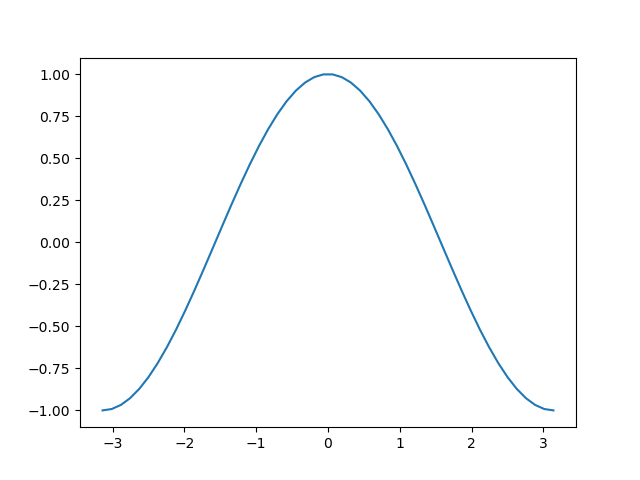
\includegraphics[width=0.7\textwidth]{./data/sen}
  \caption{Esboço do gráfico da função $y=\sen(x)$ no intervalo $[-\pi,\pi]$.}
  \label{fig:sen}
\end{figure}

Gráficos bidimensionais podem ser criados com a função \lstinline+plt.plot(x,y)+, onde \lstinline+x+ e \lstinline+y+ são \lstinline+arrays+ que fornecem os pontos cartesianos $(x_i, y_i)$ a serem plotados. Por exemplo,
\begin{lstlisting}
>>> import matplotlib.pyplot as plt
>>> x = np.linspace(-np.pi, np.pi)
>>> y = np.cos(x)
>>> plt.plot(x,y)
[<matplotlib.lines.Line2D object at 0x7f99f578a370>]
>>> plt.show()
\end{lstlisting}
produz o seguinte esboço do gráfico da função $y=\sen(x)$ no intervalo $[-\pi,\pi]$. Consulte a Figura \ref{fig:sen}.


\begin{obs}
  Matplotlib é uma poderosa ferramenta para a visualização de gráficos. Consulte a galeria de exemplos no seu site oficial
  \begin{center}
    \url{https://matplotlib.org/stable/gallery/index.html}
  \end{center}
\end{obs}

\begin{exr}
  Crie um esboço do gráfico de cada uma das seguintes funções no intervalo indicado:
  \begin{enumerate}[a)]
  \item $y = \cos(x)$, $\left[0, 2\pi\right]$
  \item $y = x^2 - x + 1$, $[-2, 2]$
  \item $y = \tg\left(\frac{\pi}{2}x\right)$, $(-1, 1)$
  \end{enumerate}
\end{exr}

%references
\nocite{*}
% \bibliographystyle{plain}
\bibliography{main}
\addcontentsline{toc}{section}{Referências Bibliográficas}

\end{document}
